% This is samplepaper.tex, a sample chapter demonstrating the
% LLNCS macro package for Springer Computer Science proceedings;
% Version 2.20 of 2017/10/04
%
\documentclass[runningheads]{llncs}
%
\usepackage{float}
\usepackage{xspace}
\usepackage{graphicx}
\graphicspath{{./imgs/}}
\usepackage{comment}
% Used for displaying a sample figure. If possible, figure files should
% be included in EPS format.
%
% If you use the hyperref package, please uncomment the following line
% to display URLs in blue roman font according to Springer's eBook style:
% \renewcommand\UrlFont{\color{blue}\rmfamily}


% nice looking audit titles
\newcommand{\Minerva}{\textsc{Minerva}\xspace}
\newcommand{\B}{{{B2}}\xspace}
\newcommand{\R}{{{R2}}\xspace}
\newcommand{\BRAVO}{\textsc{Bravo}\xspace}



\begin{document}
%
\title{Multiple Round Ballot Polling Risk-Limiting Audit Simulations}
%add \thanks{} within the title brackets if want to refer to supporting organization ^^
%
%\titlerunning{Abbreviated paper title}
% If the paper title is too long for the running head, you can set
% an abbreviated paper title here
%
\begin{comment}
\author{First Author\inst{1}\orcidID{0000-1111-2222-3333} \and
Second Author\inst{2,3}\orcidID{1111-2222-3333-4444} \and
Third Author\inst{3}\orcidID{2222--3333-4444-5555}}
%
\authorrunning{F. Author et al.}
% First names are abbreviated in the running head.
% If there are more than two authors, 'et al.' is used.
%
\institute{Princeton University, Princeton NJ 08544, USA \and
Springer Heidelberg, Tiergartenstr. 17, 69121 Heidelberg, Germany
\email{lncs@springer.com}\\
\url{http://www.springer.com/gp/computer-science/lncs} \and
ABC Institute, Rupert-Karls-University Heidelberg, Heidelberg, Germany\\
\email{\{abc,lncs\}@uni-heidelberg.de}}
%
\end{comment}
\maketitle              % typeset the header of the contribution
%
\begin{abstract}
    Risk-Limiting Audits (RLAs) guarantee with known probability 
    that if the outcome of an 
    election is incorrectly announced, it will be detected, 
    and a full hand recount will be performed. 
    In Ballot-polling RLAs, samples of ballots are drawn and tallied.
    In this paper we present an audit simulation framework
    that can be used to support theoretical results of audits.
    We present such experimental results for multiple round 
    ballot-polling RLAs.
    \BRAVO [citation] has long been the standard ballot-polling RLA,
    while \Minerva was recently introduced with the claim
    that fewer ballots on average are necessary to conclude 
    an audit.
    [Minerva paper] presented experimental
    results for one round audits, and here
    we present results
    from simulations of multiple round audits using \Minerva 
    as well as \BRAVO 
    (both Selection-Ordered 
    \BRAVO and End-of-Round \BRAVO).
    The simulation results agree within reasonable error with
    the mathematical properties claimed in [Minerva paper].
    On average, \BRAVO audits are unnecessarily conservative 
    while \Minerva audits stop with fewer ballots. We also
    present details on software implementing \Minerva and
    the simulations themselves.

\keywords{Risk-limiting audit  \and Ballot polling audit}
\end{abstract}
%
%
%

\section{Introduction: B2 and R2 Ballot Polling RLAs}
In ballot-polling RLAs, samples of ballots are drawn and tallied
in rounds
after each of which a statistical measure determines whether to
continue. 
Some ballot-polling audits (B2 audits) 
are designed to make a stopping decision
after each individual ballot is sampled.
Other ballot-polling audits (R2 audits) assume many ballots are drawn
at once and make a stopping decision at the conclusion of each 
so-called round.
In practice, election officials draw many ballots at once.
For this reason, R2 audits are used or B2 audits are applied to 
rounds.
\BRAVO is a B2 audit. 
When an audit is performed in rounds, \BRAVO can have its
stopping condition applied once at the end of each round: End-of Round (EoR) \BRAVO.
This method ignores the possibility of stopping earlier in the 
sample and thus requires more ballots on average to sample.
Alternatively, the order of ballots in the sample can be tracked
by election officials and the B2 \BRAVO stopping condition can 
be applied retroactively to all subsamples: Selection-Ordered (SO) \BRAVO.
SO \BRAVO requires fewer ballots on average than EoR \BRAVO but
requies the work of tracking the order of ballots rather than
just their tally.
\Minerva was designed for R2 audits and applies its stopping rule
once for each round.
By design then, \Minerva requires fewer ballots to be sampled when 
an audit is performed in rounds.

Now we present relevant definitions.
We consider a two candidate plurality contest.
To begin we define an audit.
\begin{definition}
An audit $\mathcal{A}$ takes a sample $X$ as input and gives one of the 
following decisions
\begin{enumerate}
\item
$Correct$: the audit is complete
\item
$Uncertain$: continue the audit
\end{enumerate}
\end{definition}
All of the audits discussed in this paper are modeled as binary hypothesis tests.
Under the alternate hypothesis, $H_a$, the announced outcome is correct. 
That is, the true underlying ballot distribution is given by the announced ballot tallies.
Under the null hypothesis, $H_0$, the true outcome is a tie 
(or a the announced winner losing by one vote if there is an odd number of total ballots).
Now we define key attributes of an audit that we will consider while analyzing our simulations.
The risk of an audit is the probability that an audit stops when a tie has occurred.
\begin{definition}[Risk]
The risk $R$ of an audit $\mathcal{A}$ is
$$R(\mathcal{A})=\Pr[\mathcal{A}(X)=Correct \mid H_0]$$
\end{definition}
This leads us to the following simple definition of an $\alpha$-RLA.
\begin{definition}[Risk Limiting Audit ($\alpha$-RLA)]
An audit $\mathcal{A}$ is a Risk Limiting Audit with 
risk limit $\alpha$ iff 
$$R(\mathcal{A}) \le \alpha.$$
\end{definition}

It is useful to discuss the probability of an audit stopping in
some round, if the outcome is correctly announced.
\begin{definition}[Stopping Probability]
The stopping probability $S$ of an audit $\mathcal{A}$ in round $j$ is 
$$S_j(\mathcal{A})=\Pr[\mathcal{A}(X_j)=Correct \mid H_a]$$
\end{definition}
The notion of stopping probability can be useful for selecting round sizes.

\section{Simulator}
\subsection{Simulations to Support Theoretical Audit Properties}

The outcomes of RLAs depend on random chance; some random samples
support the alternative hypothesis more than expected, resulting in 
quick low-risk conclusions, while other samples require subsequent
rounds in order to confirm the announced results.
We can simulate random samples for various underlying ballot 
distributions by computing pseudorandom samples. 
By applying an audit's stopping condition to thousands of such
simulated samples, the average behavior of the simulated
audits will tend towards the true behavior of the audit.
In this way, we can examine whether theoretical claims about an audit are
actually correct.

\subsection{Software for Simulations}
Our open source audit software library r2b2 [link] has implementations of several ballot polling risk-limiting audits as well as a simulator, 
all written in Python.
For each of these audits, the software can evaluate the stopping condition for a given sample and can give estimates
of the minimum round size to achieve a desired stopping probability. 
For a given audit and random seed, the simulator draws random samples using the pseudorandom number generator, [need to check].
Ballots can be sampled from any distribution of the users choosing. 
It is often useful to consider the distribution of ballots corresponding to a tie and the 
distribution of ballots corresponding with the announced results; these are the distributions represented
by the null and alternative hypotheses.
After drawing a sample, the simulator then evaluates the given audit's stopping condition for this simulated sample.
If the audit stops, the simulation stops, and if the audit continues, the simulation draws another round. 
The abstract simulator class does not prescribe any one method for choosing round sizes. 
We implement several classes to support various round size choices: 
round sizes from an estimate to achieve a desired probability of stopping, 
predetermined round sizes, and random round sizes. 

\section{Simulation Results}

For this paper, we simulated audits for 
the 2020 Presidential election
in all US states whose margin was at least $5\%$.
Round sizes increase roughly proportional to the inverse
square of the margin, so 
smaller margins are computationally much more expensive to simulate.
For each of these states, we simulated 
$10,000=10^4$ audits with the announced
underyling ballot distribution
and an additional $10,000=10^4$ audits with a tie
as the underlying ballot distribution.
These are reasonable choices for inital simulation experiments
because most audits frame the stopping decision as a binary
hypothesis test where the null hypothesis assumes an underyling tie
and the alternative hypothesis assumes the announced distribution.
A standard first round size in ballot-polling audits
has been one which achieves a $90\%$ probability
of stopping, and we chose round sizes to reflect this standard
in our simulations.
We ran our simulations for up to five rounds.
With a $90\%$ stopping probability, 
an audit only has a $a$ probablity of not stopping
by the end of the fifth round, assuming the outcome was correctly
announced.

\subsection{End-of-Round \BRAVO}
For the EoR \BRAVO simulations, our software estimated and used for each round
the minimum round size that would achieve a $90\%$ probability of stopping.
For the simulations with the announced outcome as the underlying
ballot distribution, for each round $j$ we computed the proportion of audits 
that stopped in round $j$ among those that had not stopped before round $j$.

\begin{figure}[H]
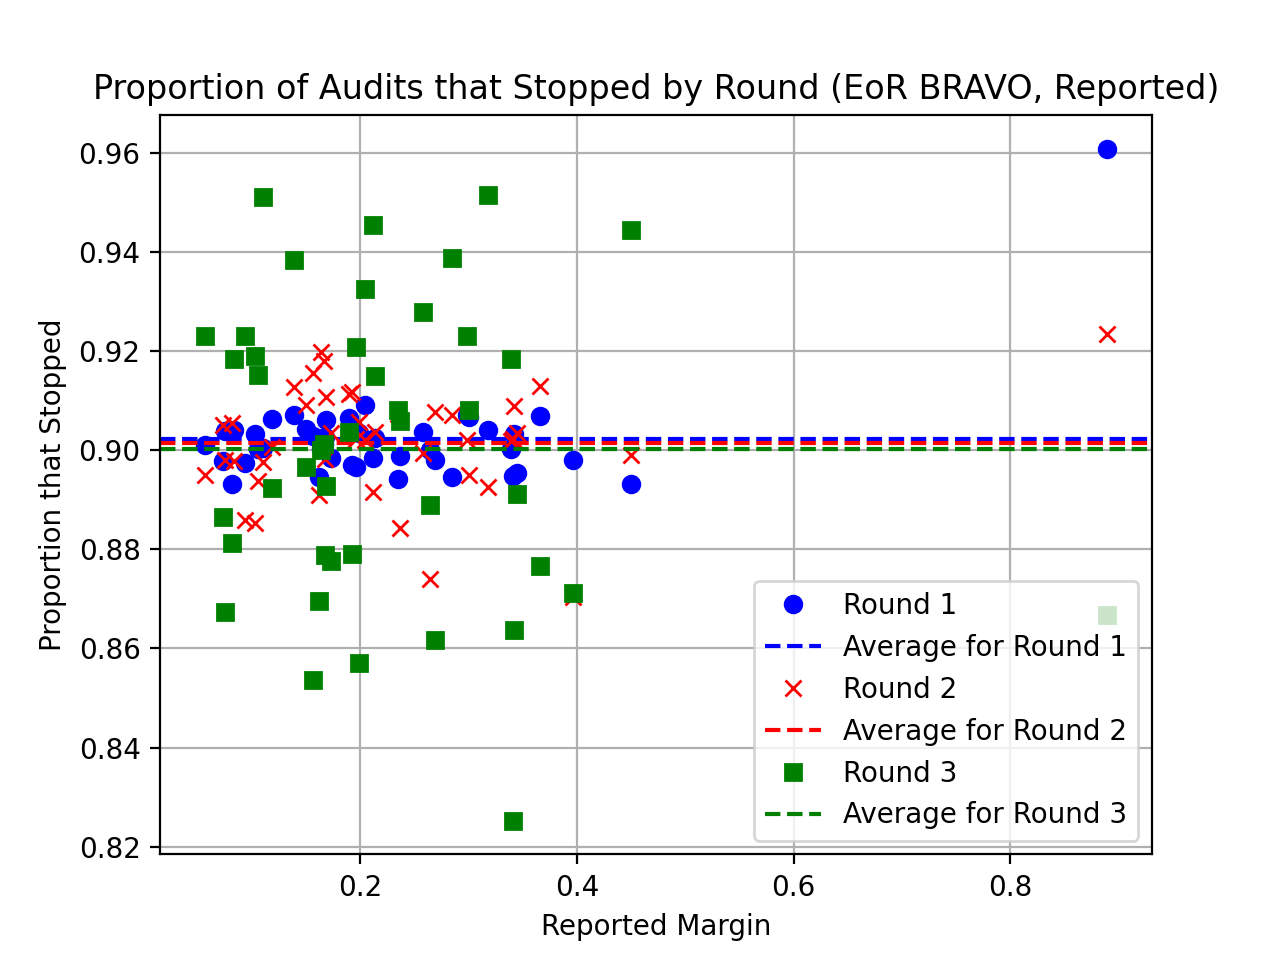
\includegraphics[width=\textwidth]{eor_bravo_90perc_10^4_corrected/sprob_first_three.png}\caption{
For the first three rounds of the EoR \BRAVO simulations, this plot shows the proportion of audits that stopped in the $j$th round
to all audits which had not yet stopped before the $j$th round.}
\label{fig:eor_bravo_sprob}
\end{figure}

In Figure \ref{fig:eor_bravo_sprob}, we display proportions for only the first three rounds
since very few audits, $(.1)^{j-1}\cdot(10^4)$ on average, 
make it to the $jth$ round.
As  a result, the proportions are based on an exponentially smaller dataset in each round.
The proportions shown in Figure \ref{fig:eor_bravo_sprob} give an estimate
of the true probability of an EOR \BRAVO audit stopping in the $j$th round,
given that it has not already stopped in a previous round. 
In \ref{fig:eor_bravo_sprob}, we see that, especially in earlier rounds for which 
the values are more representative of true audit behavior, 
our predictions are accurate.
In particular, the average across all margins is just above $.9=90\%$ for
all three rounds.

The risk of this audit, across all $5$ rounds, is an important metric since it determines whether an audit is risk-limiting.
Therefore, we now consider the proportion of audits that stopped with an underlying tie.
This proportion, for a risk-limiting audit, should approach a value less than the risk limit, $0.1$, as more audits are performed.

\begin{figure}[H]
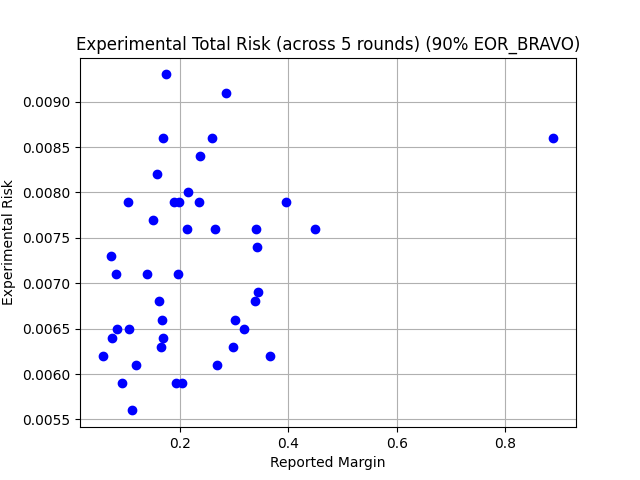
\includegraphics[width=\textwidth]{eor_bravo_90perc_10^4_corrected/total_risk.png}
\caption{For each state margin, this plot shows
the proportion of EOR \BRAVO audits with an underlying
tie that stopped.}
\label{fig:eor_bravo_risk}
\end{figure}

Figure~\ref{fig:eor_bravo_risk} makes it clear that the risk of EOR \BRAVO is roughly
an order of magnitude less than the risk limit. 
That is, on average, roughly $10$ times more audits could have stopped 
with the audit still meeting the risk limit.
These simulations support the claim made in [\Minerva paper]
that EOR \BRAVO is unnecessarily conservative and thus requires
more ballots on average.

% \subsection{Selection-Ordered BRAVO}
% next_sample_size code is slow... tie simulations running still!

\subsection{\Minerva Simulations}
For \Minerva, it has not been shown that round sizes can be chosen
during the audit. That is, an adversary with knowledge of the history
of the audit may be able to choose round sizes which cause the 
risk of the audit to exceed the risk limit.
For this reason, we have to choose the round sizes of a \Minerva 
audit a priori.
For this paper, we consider two choices of round sizes.
For both, we estimate and then use the minimum first round size 
which achieves
a $90\%$ probability of stopping.
Then, for subsequent rounds, we either (i) 
draw the same number of ballots in each round or (ii)
multiply the previous round size by a factor of $1.5$ and 
sample this many new ballots.
We consider the case of drawing samples of the same size
because it may reflect a practical way to continue an
audit; if election officials have selected some first round size within
reasonable logistical bounds, drawing the same number of 
ballots in subsequent rounds may be practical.
We also consider round sizes with samples increasing by a multiple
of $1.5$ because this multiple gives a very rough approximation of 
round sizes with a $90\%$ probability of stopping.

\subsubsection{Round Sizes with Multiple of $1.0$}

As with the preceding simulations, we ran $10,000=10^4$ trials
per state for both the underlying tie and underlying reported
outcome.

\begin{figure}[H]
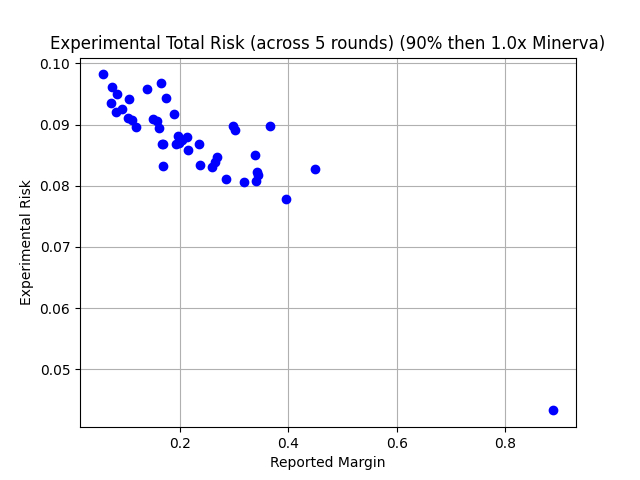
\includegraphics[width=\textwidth]{minerva_multiround_1x_10^4/total_risk.png}
\caption{This plot shows, for each state's margin, the proportion of audits that stopped of
all $10^4$ audits with an underlying tie in the simulations with a round size multiple of $1.0$.}
\label{fig:minerva1_risk}
\end{figure}

Notice in Figure \ref{fig:minerva1_risk} that all simulations for a tie had a proportion of audits that stopped less than $.1$, the risk limit, supporting
the claim that \Minerva is a risk limiting audit. 
Unlike EOR \BRAVO, the experimental risks here are much closer to the risk limit,
showing that \Minerva stops on average with a less conservative risk; \Minerva is sharper.

\begin{figure}[H]
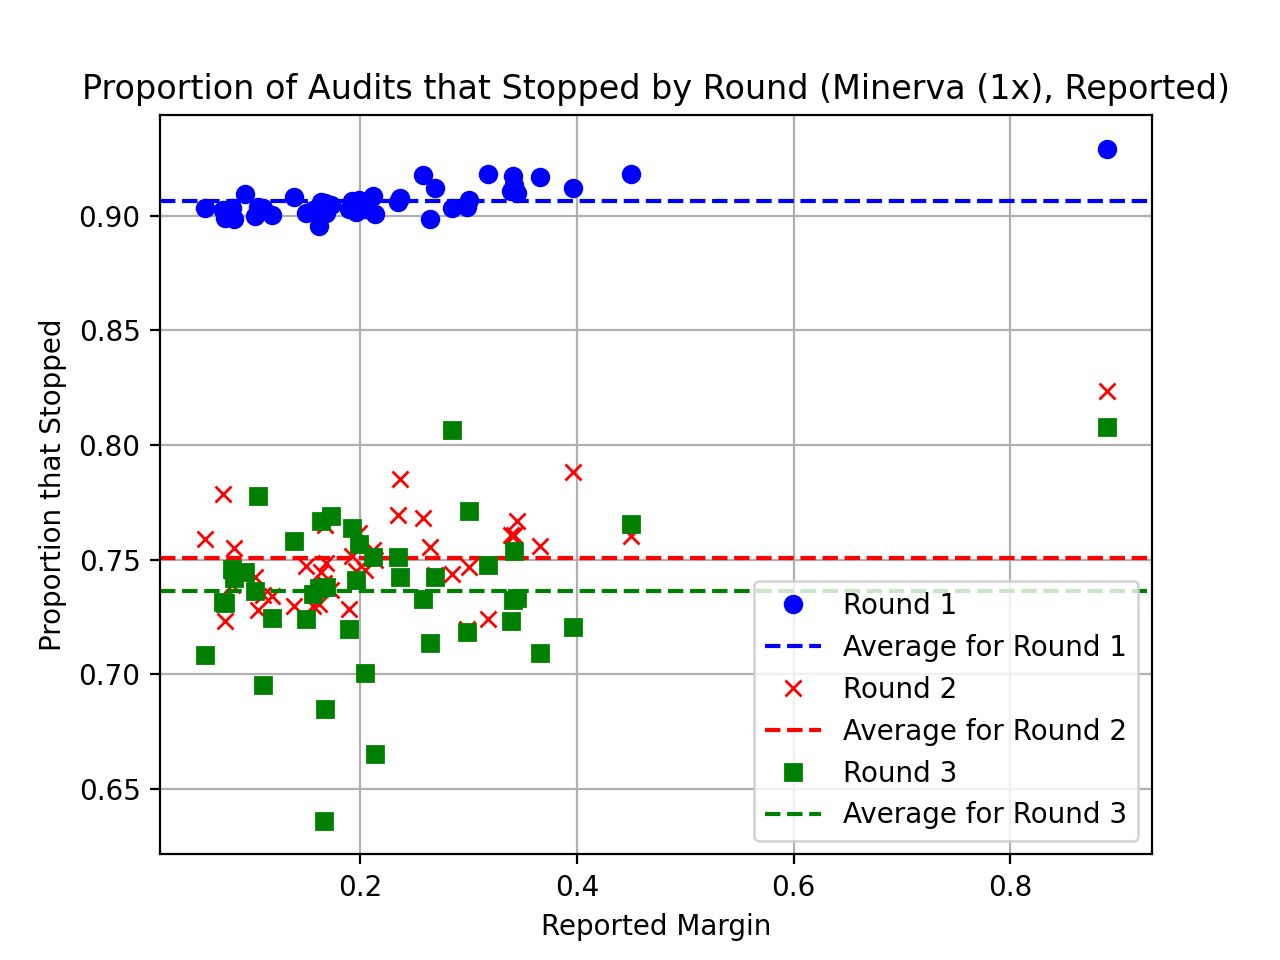
\includegraphics[width=\textwidth]{minerva_multiround_1x_10^4/sprobs_first_three.png}
\caption{This plot shows, for each state's margin, the proportion of audits that stopped of
all $10^4$ audits with the announced results as the underlying distribution
in the \Minerva simulations with a round size multiple of $1.0$.}
\label{fig:minerva1_sprob}
\end{figure}

Figure~\ref{fig:minerva1_sprob} shows that the round size estimate for the first round achieved the desired
stopping probability of $90\%$. For subsequent rounds, the multiplier of $1.5$ did not consistently achieve $90\%$ stopping
probability, but it was within  roughly $10\%$. 

\subsubsection{Round Sizes with Multiple of $1.5$}

%For the Minerva simulations with a round size multiple of $1.5$,
%we increased the number of simulations to $10^6$ per state for 
%both an underlying tie and underlying announced outcome. 

%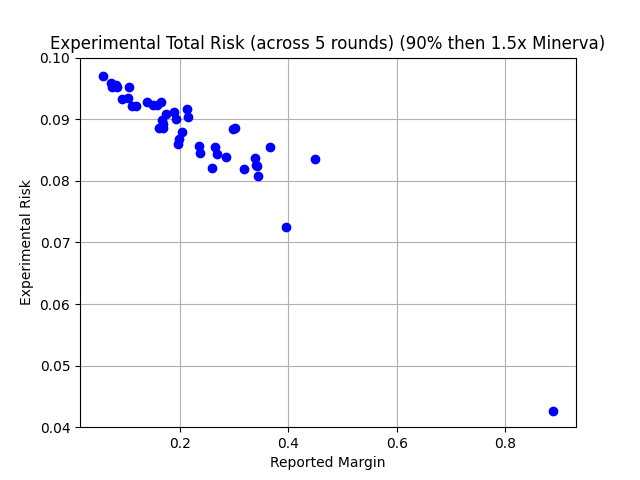
\includegraphics[width=\textwidth]{minerva_multiround_1p5x_10^6/total_risk.png}

\begin{figure}[H]
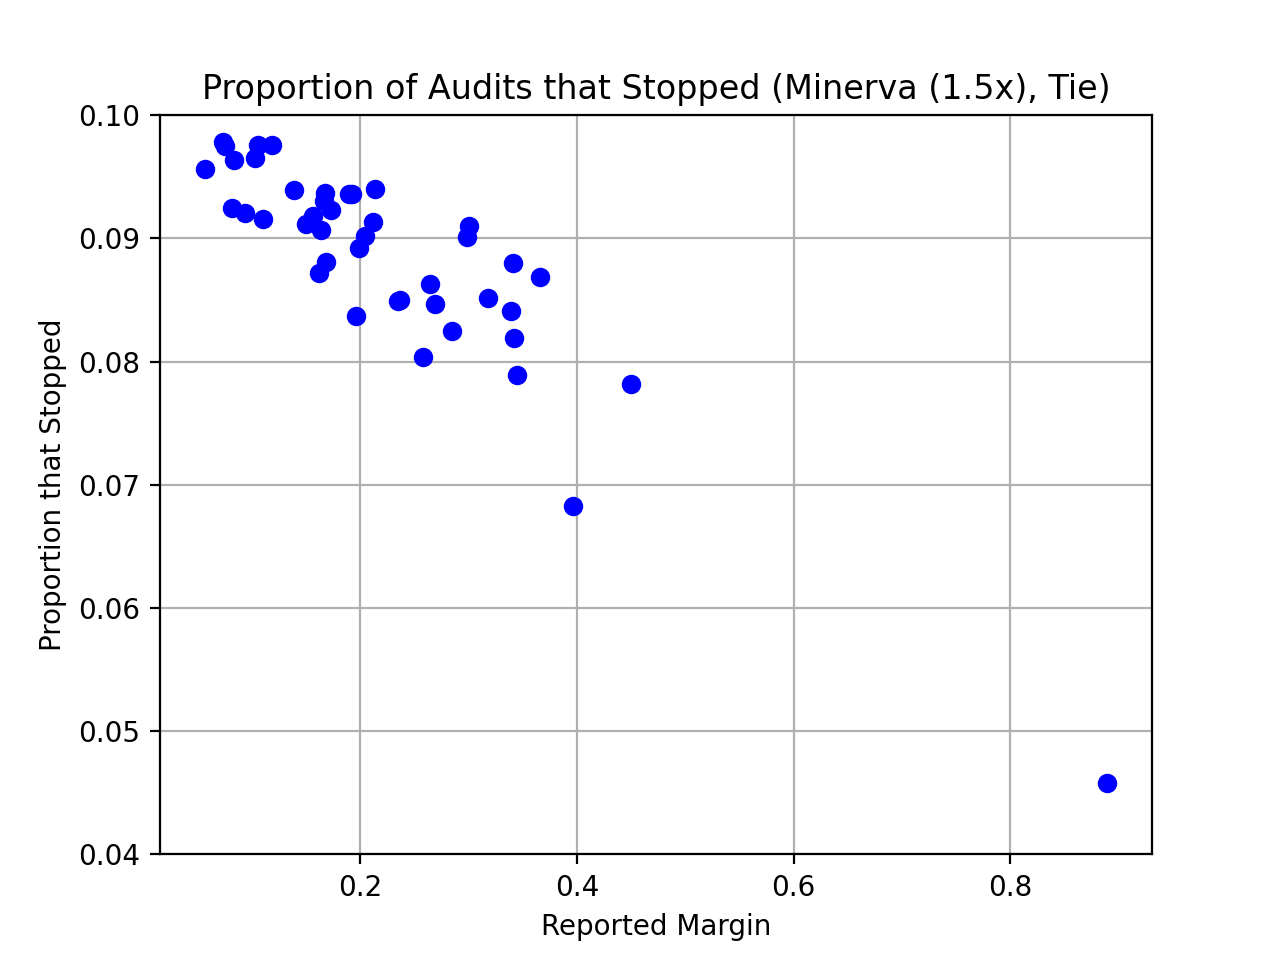
\includegraphics[width=\textwidth]{minerva_multiround_1p5x_10^4/total_risk.png}
\caption{This plot shows, for each state's margin, the proportion of audits that stopped of
all $10^4$ audits with an underlying tie in the simulations with a round size multiple of $1.5$.}
\label{fig:minerva1p5_risk}
\end{figure}

Figure~\ref{fig:minerva1p5_risk} shows, for each state's margin, the proportion of audits that stopped of
all $10^4$ audits with an underlying tie in the simulations with a round size multiple of $1.5$.

\begin{figure}[H]
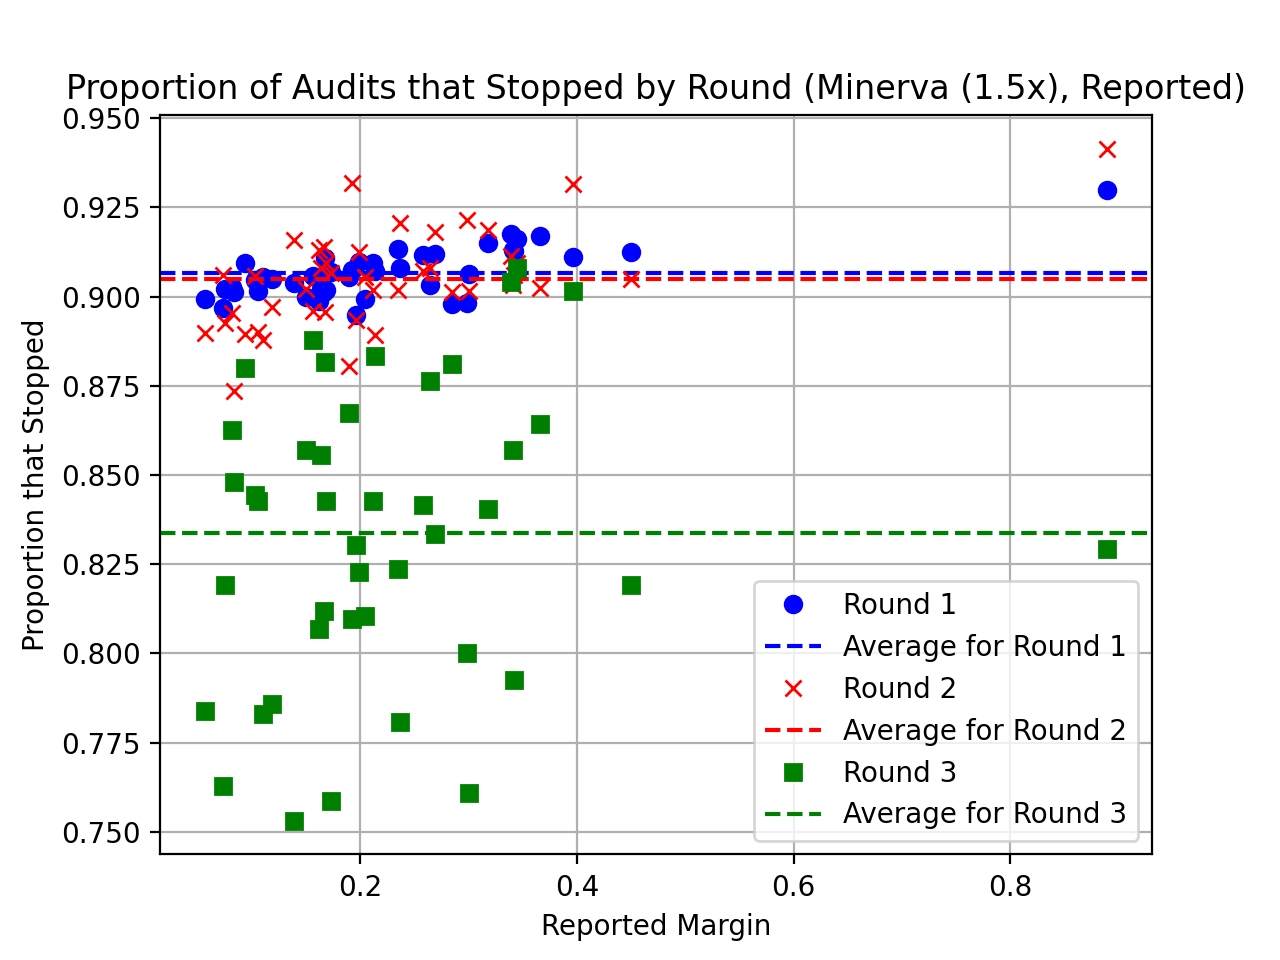
\includegraphics[width=\textwidth]{minerva_multiround_1p5x_10^4/sprobs_first_three.png}
\caption{This plot shows, for each state's margin, the proportion of audits that stopped in each round
with the announced results as the underlying distribution
in the \Minerva simulations with a round size multiple of $1.5$.}
\label{fig:minerva1p5_sprob}
\end{figure}

Figure~\ref{fig:minerva1p5_sprob} shows that the round size estimate for the first round achieved the desired
stopping probability of $90\%$. For subsequent rounds, the multiplier of $1.5$ did not consistently achieve $90\%$ stopping
probability, but it was within  roughly $10\%$. 
% we could suggest that predicting accurate multiples is possible (same curve rather than line)







%
% ---- Bibliography ----
%
% BibTeX users should specify bibliography style 'splncs04'.
% References will then be sorted and formatted in the correct style.
%
% \bibliographystyle{splncs04}
% \bibliography{mybibliography}
%
\begin{thebibliography}{8}
\bibitem{ref_article1}
Author, F.: Article title. Journal \textbf{2}(5), 99--110 (2016)

\bibitem{ref_lncs1}
Author, F., Author, S.: Title of a proceedings paper. In: Editor,
F., Editor, S. (eds.) CONFERENCE 2016, LNCS, vol. 9999, pp. 1--13.
Springer, Heidelberg (2016). \doi{10.10007/1234567890}

\bibitem{ref_book1}
Author, F., Author, S., Author, T.: Book title. 2nd edn. Publisher,
Location (1999)

\bibitem{ref_proc1}
Author, A.-B.: Contribution title. In: 9th International Proceedings
on Proceedings, pp. 1--2. Publisher, Location (2010)

\bibitem{ref_url1}
LNCS Homepage, \url{http://www.springer.com/lncs}. Last accessed 4
Oct 2017
\end{thebibliography}
\end{document}
